\documentclass[final]{book}
\newcommand{\doctitle}{HSA Runtime Programmer's Reference Manual}
\newcommand{\docversion}{0.182}

% Needed so characters such as underscore are recognized in PDF
% viewers. Otherwise searching for say `hsa_open` produces no
% results
\usepackage[T1]{fontenc}

% If draft, use narrow margins (better for printing)
\usepackage{ifdraft}
% \ifdraft{\usepackage[top=.5cm,bottom=.5cm,left=.5cm,right=.5cm]{geometry}}
%          {\usepackage[top=2.5cm,bottom=2.5cm,left=2.5cm,right=2.5cm]{geometry}}
\usepackage[top=2.5cm,bottom=2.5cm,left=2.5cm,right=2.5cm]{geometry}

\usepackage[toc,page]{appendix}
\usepackage[usenames,dvipsnames,svgnames,table]{xcolor}
  \definecolor{lightgray}{gray}{0.9}
\usepackage{makeidx}
\usepackage[final]{graphicx}
\usepackage{sidecap}
\usepackage{float}

% overwrite global draft option so the source is shown in draft mode
\usepackage[final]{listings}

% allow tables across page breaks
\usepackage{longtable}

% Use Tikz for simple diagrams
\usepackage{tikz}
\usetikzlibrary{arrows,automata,positioning,chains}
\tikzset{
    % define global arrow tip format
    >=angle 45}

% allows width arithmetic, currently used in the LaTeX generated by xml2py
\usepackage{calc}
% allow usage of underscore w/o resorting to underscore package
% the underscore package imposes more restrictions on where underscores still
% cannot be used (e.g.: labels)
\catcode`\_=12

\usepackage{ifthen}
\usepackage{textcomp}

% inline enumerations and itemizes in the paragraph instead of breaking
\usepackage{paralist}

% Customizable headers/footers
\usepackage{fancyhdr}

% add API index. Note that 'imakeidx' works within Latex (unlike 'makeidx', which
% requires running 'makeindex' from command line)
\usepackage{imakeidx}
\makeindex[name=api,title=Index - Core APIs,columns=1,intoc]
\makeindex[name=ext,title=Index - Extension APIs,columns=1,intoc]

% Times font definitions
\usepackage{times}

% allows customization of description environment (margin, indentation, etc.)
\usepackage{enumitem}

% colored boxes with plenty of configuration properties
\usepackage{tcolorbox}
  % allow page breaks within boxes
  \tcbuselibrary{breakable}

\usepackage{ifpdf}
\ifpdf
\usepackage[pdftex,
            bookmarks,
            final, % use links even if the document is draft
            pagebackref=true,
            pdfpagemode=UseOutlines, % generate index
            linktoc=all,  % sections and subsections linked
            colorlinks=true,
            linkcolor=black,
            unicode
           ]{hyperref}
\else
\usepackage[ps2pdf,
            bookmarks,
            final, % use links even if the document is draft
            pdfpagemode=UseOutlines, % generate index
            linktoc=all,  % sections and subsections linked
            pagebackref=true,
            colorlinks=true,
            linkcolor=black,
            unicode
           ]{hyperref}
\usepackage{pspicture}
\fi

\lstset{language=C++,
        inputencoding=utf8,
        basicstyle=\small,
        breaklines=true,
        breakatwhitespace=true,
        tabsize=4,
        showstringspaces=false,
        frame=none,
        backgroundcolor=\color{lightgray},
        keywordstyle=,
        emphstyle={\textbf},
        commentstyle=\color{ForestGreen},
        morecomment=[l][\color{green}]{\#}
}
% include automatically-generated Listing commands
\input{api/altlatex/listings}

% formatting of arguments, function names, types, etc.
% remember to add this commands to the safe command list of Latexdiff so
% it includes them in the diff algorithm
\newcommand{\hsaarg}[1]{\textit{#1}}
\newcommand{\reffun}[1]{\textbf{#1}}
\newcommand{\refarg}[1]{\textit{#1}}
\newcommand{\reffld}[1]{\textit{#1}}
\newcommand{\reftyp}[1]{#1}
\newcommand{\refenu}[1]{\reftyp{#1}}
\newcommand{\refhsl}[1]{\reffun{#1}}

% allows string comparison, which is used to match \hsaref arguments
\usepackage{pdftexcmds}
% Automatically generated file containing all the definitions in the header that
% can be referenced via \hsaref commands
\input{api/altlatex/commands}

% every section in a new page
\usepackage{etoolbox}
\pretocmd{\section}{%
  \ifnum\value{section}=0 \else\clearpage\fi
}{}{}

% define marginparwidth so todonotes renders properly
\setlength{\marginparwidth}{2cm}
\usepackage[obeyDraft,obeyFinal,textsize=scriptsize]{todonotes}

% Alter some LaTeX defaults for better treatment of figures:
% See p.105 of "TeX Unbound" for suggested values.
% See pp. 199-200 of Lamport's "LaTeX" book for details.
%   General parameters, for ALL pages:
\renewcommand{\topfraction}{0.9}	% max fraction of floats at top
\renewcommand{\bottomfraction}{0.8}	% max fraction of floats at bottom
%   Parameters for TEXT pages (not float pages):
\setcounter{topnumber}{2}
\setcounter{bottomnumber}{2}
\setcounter{totalnumber}{4}     % 2 may work better
\setcounter{dbltopnumber}{2}    % for 2-column pages
\renewcommand{\dbltopfraction}{0.9}	% fit big float above 2-col. text
\renewcommand{\textfraction}{0.07}	% allow minimal text w. figs
%   Parameters for FLOAT pages (not text pages):
\renewcommand{\floatpagefraction}{0.7}	% require fuller float pages
% N.B.: floatpagefraction MUST be less than topfraction !!
\renewcommand{\dblfloatpagefraction}{0.7}	% require fuller float pages

%%%%%%%%%%%%%%%%%%%%%%%%%%%%%%%%%%%%%%%%%%%%%%%%%

% push footer a little further away
\setlength{\footskip}{35pt}

% Side notes. One command per author
\newcommand{\mariotodo}[1]{\todo[color=CarnationPink]{#1}}

% Increase paragraph separation
\setlength{\parskip}{2mm}

% no indentation
\setlength{\parindent}{0cm}

% number (sub)sections up to level 3
\setcounter{secnumdepth}{3}

\makeindex
\setcounter{tocdepth}{3}
\renewcommand{\footrulewidth}{0.4pt}
\renewcommand{\familydefault}{\sfdefault}

\RequirePackage[normalem]{ulem} %DIF PREAMBLE
\newenvironment{DIFnomarkup}{}{}

% header and footer layout
\newcommand{\hfstyle}{
\fancyhf{} % clear all header and footer fields
\fancyfoot[LE,RO]{\scriptsize{\thepage}}
\fancyfoot[LO,RE]{\scriptsize{\doctitle$\:$v\docversion $\:$-$\:$\today}}
\fancyhead[RE]{\scriptsize{\nouppercase{\leftmark}}}
\fancyhead[LO]{\scriptsize{\nouppercase{\rightmark}}}
\renewcommand{\headrulewidth}{0pt}
\renewcommand{\footrulewidth}{0pt}
}

\pagestyle{fancy}
\renewcommand{\chaptermark}[1]{\markboth{#1}{}}
\renewcommand{\sectionmark}[1]{\markright{#1}{}}
\hfstyle{}

% plain style is identical to fancy style. This avoids different formatting in
% the first page of every chapter, for example.
\fancypagestyle{plain}{\hfstyle{}}

\begin{document}

\hypersetup{pageanchor=false,citecolor=black}
\begin{titlepage}

\includegraphics[width=.5\textwidth]{fig/foundation.png}
\vspace*{7cm}
\begin{center}
{\Large \doctitle\\[1ex]\large\docversion}\\
\vspace*{1cm}
\vspace*{0.5cm}
{\small \today}\\
\vspace*{0.5cm}
{\small Draft}\\
\end{center}
\end{titlepage}
\thispagestyle{empty} {\textcopyright 2013-2014 HSA Foundation. All rights
  reserved.}


The contents of this document are provided in connection with the HSA Foundation
specifications. This specification is protected by copyright laws and contains
material proprietary to the HSA Foundation. It or any components may not be
reproduced, republished, distributed, transmitted, displayed, broadcast or
otherwise exploited in any manner without the express prior written permission
of HSA Foundation. You may use this specification for implementing the
functionality therein, without altering or removing any trademark, copyright or
other notice from the specification, but the receipt or possession of this
specification does not convey any rights to reproduce, disclose, or distribute
its contents, or to manufacture, use, or sell anything that it may describe, in
whole or in part.

HSA Foundation grants express permission to any current Founder, Promoter,
Supporter Contributor, Academic or Associate member of HSA Foundation to copy
and redistribute UNMODIFIED versions of this specification in any fashion,
provided that NO CHARGE is made for the specification and the latest available
update of the specification for any version of the API is used whenever
possible. Such distributed specification may be re-formatted AS LONG AS the
contents of the specification are not changed in any way. The specification may
be incorporated into a product that is sold as long as such product includes
significant independent work developed by the seller. A link to the current
version of this specification on the HSA Foundation web-site should be included
whenever possible with specification distributions.

HSA Foundation makes no, and expressly disclaims any, representations or
warranties, express or implied, regarding this specification, including, without
limitation, any implied warranties of merchantability or fitness for a
particular purpose or non-infringement of any intellectual property. HSA
Foundation makes no, and expressly disclaims any, warranties, express or
implied, regarding the correctness, accuracy, completeness, timeliness, and
reliability of the specification. Under no circumstances will the HSA
Foundation, or any of its Founders, Promoters, Supporters, Academic,
Contributors, and Associates members or their respective partners, officers,
directors, employees, agents or representatives be liable for any damages,
whether direct, indirect, special or consequential damages for lost revenues,
lost profits, or otherwise, arising from or in connection with these materials.

\clearpage \pagenumbering{roman}
\addtocontents{toc}{}
\tableofcontents
\clearpage

\pagenumbering{arabic}
\setcounter{page}{1}

\chapter{Introduction} \label{index}\hypertarget{index}{}
\hypertarget{overview}{}\section{Overview}\label{overview}

Recent heterogeneous system designs have integrated CPU, GPU, and other
accelerator devices into a single platform with a shared high-bandwidth memory
system.  Specialized accelerators now complement general purpose CPU chips and
are used to provide both power and performance benefits.  These
heterogeneous designs are now widely used in many computing markets including
cellphones, tablets, personal computers, and game consoles. The Heterogeneous
System Architecture (HSA) builds on the close physical integration of
accelerators that is already occurring in the marketplace, and takes the next
step by defining standards for uniting the accelerators architecturally. The HSA
specifications include requirements for virtual memory, memory coherency,
architected dispatch mechanisms, and power-efficient signals. HSA refers to
these accelerators as "components".

The system architecture defines a consistent base for building portable
applications that access the power and performance benefits of the dedicated HSA
components. Many of these components, including GPUs and DSPs, are capable and
flexible processors that have been extended with special hardware for
accelerating parallel code. Historically these devices have been difficult to
program due to a need for specialized or proprietary programming languages. HSA
aims to bring the benefits of these components to mainstream programming
languages using similar or identical syntax to that which is provided for
programming multi-core CPUs.

In addition to the system architecture, HSA defines a portable, low-level,
compiler intermediate language called ``HSAIL''.  A high-level compiler generates
the HSAIL for the parallel regions of code. A low-level compiler called the
``finalizer'' translates the intermediate HSAIL to target machine code.  Each 
HSA component provides its own implementation of the finalizer.  For more
information on HSAIL, refer to the HSA Programmer's Reference Manual~\cite{prm}.

The final piece of the puzzle is the HSA Runtime API.  The runtime is a thin,
user-mode API that provides the interfaces necessary for the host to launch
compute kernels to the available components. This document describes the
architecture and APIs for the HSA Runtime. Key sections of the runtime API
include:
\begin{itemize}
\item Error Handling
\item Runtime initialization and shutdown
\item Topology discovery
\item Signals and synchronization
\item Architected dispatch
\item Memory management
\end{itemize}

The remainder of this document describes the HSA software architecture and
execution model, and includes functional descriptions for all of the HSA APIs
and associated data structures.

\begin{figure}
  \centering
  \tikzstyle{lang}=[rectangle,draw,fill=black!30,align=center,minimum width=1.25cm,minimum height=.75cm]
  \tikzstyle{hsa}=[rectangle,draw,fill=black!10,align=center,minimum height=.75cm]
  \tikzstyle{comp}=[rectangle,draw,minimum height=.75cm]
  \begin{tikzpicture}[thick,auto, node distance=1.5cm]
    \scriptsize
    \node[lang] (l0) {OpenCL\texttrademark \\ app};
    \node[lang,below of=l0] (r0) {OpenCL\texttrademark \\ runtime};

    \node[lang,right of=l0] (l1) {Java \\ app};
    \node[lang,below of=l1] (r1) {JVM};

    \node[inner sep=0,below right=.75cm of l1] (k) {...};

    \node[lang,above right=.75cm of k] (l2) {OpenMP \\ app};
    \node[lang,below of=l2] (r2) {OpenMP \\ runtime};

    \node[lang,right of=l2] (l3) {DSL \\ app};
    \node[lang,below of=l3] (r3) {DSL \\ runtime};

    \node[hsa,minimum width=3.5cm,below=2cm of k] (h) {HSA runtime};
    \node[hsa,minimum width=3cm,right=1.5cm of h] (hf) {HSA finalizer};
    \tiny
    \node[comp, below=.75cm of h.west,anchor=west] (c1) {HSA component 1};
    \node[below=.5cm of h.south,anchor=south]       (cAny)  {...};
    \node[comp,below=.75cm of h.east,anchor=east]  (cN) {HSA component N};

    \path[->]
       (l0) edge (r0)
       (l1) edge (r1)
       (l2) edge (r2)
       (l3) edge (r3)
       (r0.south) edge (h)
       (r1) edge (h)
       (r2) edge (h)
       (r3.south) edge (h)
       (h) edge[dashed] (hf)
    ;
  \end{tikzpicture}
  \caption{HSA Software Architecture}
  \label{fig:swarch}
\end{figure}

Figure~\ref{fig:swarch} shows how the HSA Runtime fits into a typical software
architecture stack. At the top of the stack is a programming model such as
OpenCL\texttrademark, Java, OpenMP, or a domain-specific language (DSL). The
programming model must include some way to indicate a parallel region that can
be accelerated. For example, OpenCL has calls to \texttt{clEnqueueNDRangeKernel}
with associated kernels and grid ranges. Java defines stream and lambda APIs,
which provide support for both multi-core CPUs and HSA Components. OpenMP
contains OMP pragmas that mark loops for parallel computing and that control 
other aspects of the parallel implementation. Other programming models can also 
build on this same infrastructure.

The language compiler is responsible for generating HSAIL code for the parallel
regions of code. The code can be pre-compiled before runtime or compiled at 
runtime. A high-level compiler can generate the HSAIL before runtime, in which 
case when the application loads the finalizer converts the HSAIL to machine 
code for the target machine. Another option is to run the finalizer when 
the applications is built, in which case the resulting binary includes the machine 
code for the target architecture. The HSA Finalizer is an optional component of 
the HSA Runtime, which can reduce the footprint of the HSA software on systems 
where the finalization is done before runtime.

Each language also includes a "language runtime" that connects the language
implementation to the HSA Runtime. When the language compiler generates code for
a parallel region, it will include calls to the HSA Runtime to set up and
dispatch the parallel region to the HSA Component. The language runtime is also
responsible for initializing HSA, selecting target devices, creating execution
queues, managing memory - and may use other HSA Runtime features as well.
A runtime implementation may provide optional extensions. Applications can
query the runtime to determine which extensions are available. This document 
describes the extensions for the Finalizer and for Images and Samplers.

The API for the HSA Runtime is standard across all HSA vendors, such that
languages that use the HSA Runtime can execute on the different vendor's
platforms that support the API. Each vendor is responsible for supplying their 
own HSA Runtime implementation that supports all of the HSA components in the 
vendor's platform. HSA does not provide a mechanism to combine runtimes from 
different vendors. The implementation of the HSA Runtime may include 
kernel-level components (required for some hardware components) or may be entirely 
user-space (for example, simulators or CPU implementations).

Figure~\ref{fig:swarch} shows the ``AQL'' (Architected Queuing
Language) path that application runtimes use to send commands directly to
HSA components. For more information on AQL, refer to Section~\ref{sec:aql}.


\section{Execution Model}\label{executionmodel}

The HSA runtime exposes several details of the HSA hardware, including
architected dispatches. The overall goal of the core runtime design is to
provide a high-performance dispatch mechanism that is portable across multiple
HSA vendor architectures. Two vendors with the same host ISA but different
HSA-compliant GPUs will be able to run the same unmodified application binary 
file(s), because they support the HSA-architected AQL interface and supply a 
library that implements the architected core runtime API.

The HSA core runtime takes advantage of architected dispatch. Architected 
dispatch is the key feature in an HSA system that enables a user-level 
application to directly issue commands to the HSA Component hardware. 
Architected dispatch differentiates the HSA runtime from other higher-level 
runtime systems and programming models: other runtime systems provide 
software APIs for setting arguments and launching kernels, while HSA architects 
these at the hardware and specification level. The main advantage of architected 
dispatch is that the dispatch mechanism is architected at the HSA hardware level 
which means that an application can use regular memory operations and the 
wrapper API provided by the runtime to launch a kernel. The application creates 
user mode queues and AQL packets in memory, and then signals the HSA component 
to begin executing the packet using lightweight operations.

This section describes various features the HSA runtime provides to support 
architected dispatch, and the steps an application needs to perform in order to 
dispatch a kernel.

\subsection{Initial Setup}
One of the first steps an application must perform is agent (device) discovery. 
Agent discovery is performed after initialization of the runtime and information is
made available to the user as data structures. Section~\ref{sec:topology}
describes these \textit{topology descriptors}. 

The next step in the setup is the creation of the component queues. Queues are an 
HSA architected mechanism that submits work to the HSA component hardware. For 
more information about the interfaces for queue creation, refer to 
Section~\ref{sec:queues}. Different components may provide 
implementation-specific code under the HSA API for these functions.

% \subsection{Compilation Flow}
% Once an HSAIL program is written or generated by a higher-level compilation
% step, it needs to be \emph{assembled} to generate a BRIG. BRIG is the HSAIL
% object format and is specified in the PRM. HSA runtime defines API call to
% compile the BRIG and generate a code object that has sufficient information to
% execute the user program. The details of this compilation process and symbol
% resolution are discussed in Section~\ref{finalizerchapter}.

\subsection{Kernel Execution}
The Systems Architecture Requirements document~\cite{sar} specifies the
structure of the \emph{packets} (i.e. commands) that can be placed on the HSA
user mode queues for execution by the component hardware. The Architected 
Queuing Language (AQL) describes the format of the packets. One type of
AQL packet is a Dispatch packet. An application can create an AQL packet 
and initialize it with the code object that contains a component-specific ISA. 
% The interface for kernel arguments between the
% runtime and the kernel ISA (instruction set architecture) is also architected
% at the HSA level. This is covered in the HSAIL ABI, which specifies the
% in-memory layout of the kernarg segment. Users can determine the layout of the
% kernarg memory segment at compile time merely by examining the signature of
% the HSAIL function. The finalizer is required to support this ABI and thus
% there is no need for runtime metadata to specify the position or format of
% arguments.  This step can be done once for each AQL packet creation.

Optimized implementations can cache the result of this step and re-use the AQL
packet for subsequent launches. Care must be taken to ensure that the AQL
Dispatch packet (and the associated kernel and spill/arg/private memory) is not
re-used before the launch completes. For simple cases such as a
single-thread, synchronous launch, the AQL Dispatch packet(s) can be declared
as a static variable and initialized at the same time the code is
finalized. More complex cases might involve creating and tracking several 
Dispatch packets for a single kernel code object.

HSA hardware defines a packet process for processing these packets and a doorbell
mechanism to inform the packet processing HW that packets have been written into
the queue. The HSA runtime defines a structure and update API to inform the HW
that the Dispatch packet has been written to the queue. 

For more information on creating queues and the states of queues, refer to 
Section~\ref{sec:queues}. For more information on packet formats and the states 
of packets, refer to Section~\ref{sec:aql}. 

After a packet is written and the hardware informed by way of the doorbell, 
execution can start. Execution of a kernel happens asynchronously. An application 
can write more packets to launch other kernels in the queue. This activity can
overlap the actual execution of the kernel.

\subsection{Kernel Completion}
The architecture specification~\cite{sar} defines signals as a mechanism for
communication between different parts of an HSA system. The HSA core runtime 
defines signals as opaque objects. The API is defined to send a value to the 
signal and wait for a value at the signal. For more information on signals, 
refer to Section~\ref{sec:signals}.

The AQL Dispatch packet provides a data field that allows an application to pass 
an opaque signal. When the HSA Component hardware observes a valid signal in 
an AQL packet, it sends a value to this signal when execution of the kernel 
completes (success or error). An application can wait on this signal to determine 
kernel completion. For more information on errors, refer to 
Section~\ref{sec:error}.

\subsection{Example}
\lstinputlisting{api/first.c}

\chapter{HSA Core Programming Guide} \label{coreapi}

This chapter describes the HSA Core runtime APIs, organized by functional
area. For information on definitions that are not specific to any functionality, 
refer to Section~\ref{sec:other}.

Several operating systems allow functions to be executed when a DLL or a shared
library is loaded (for example, DLL main in Windows and GCC
\emph{constructor/destructor} attributes that allow functions to be executed
prior to main in several operating systems). Whether or not the HSA runtime
functions are allowed to be invoked in such fashion may be implementation
specific and is outside the scope of this specification.

Any header files distributed by the HSA foundation for this specification may
contain calling-convention specific prefixes such as __cdecl or __stdcall, which
are outside the scope of the API definition.

Unless otherwise stated, functions can be considered thread-safe.

\section{Initialization and Shut Down}\label{sec:init}
When an application initializes a runtime (\hsaref{hsa_init}) for the first time 
in a given process, a runtime instance is created. The instance is internally
reference counted such that multiple HSA clients within the same process do not
interfere with each other. Invoking the initialization routine $n$ times within
a process does not create $n$ runtime instances, but a unique runtime object
with an associated reference counter of $n$. Shutting down the runtime
(\hsaref{hsa_shut_down}) is equivalent to decreasing its reference counter. When
the reference counter is less than one, the runtime object ceases to exists and
any reference to it (or to any resources created while it was active) results in
undefined behavior.

\subsection{API}
\input{api/altlatex/group-initshutdown}

\section{Runtime Notifications}
\label{sec:error}

The runtime can report notifications (such as errors, and events) synchronously 
or asynchronously. The runtime uses the return value of functions in the HSA API
to pass notifications synchronously. In this case, the notification is a status 
code of type \hsaref{hsa_status_t} that indicates success or error.

The documentation of each function defines what constitutes a successful
execution. When a HSA function does not execute successfully, the returned
status code might help determining the source of the error. While a few error
conditions can be generalized to a certain degree (e.g. failure in allocating
resources) many errors can have implementation-specific explanations. For
example, operations on signals (see Section~\ref{sec:signals}) might
fail if the implementation validates the signal object on which the signals 
operate. Because the representation of a signal is specific to the 
implementation, the reported error would simply indicate that the signal is 
invalid.

The \hsaref{hsa_status_t} enumeration captures the result of any API function
that has been executed, except for accessors and mutators. Success is
represented by \hsaref{HSA_STATUS_SUCCESS}, which has a value of zero. Error
statuses are assigned positive integers and their identifiers start with the
\refenu{HSA_STATUS_ERROR} prefix. The application might use
\hsaref{hsa_status_string} to obtain a string describing a status code.

The runtime passes \textit{asynchronous} notifications in a different 
fashion. When the runtime detects an asynchronous event, the runtime invokes a
user-defined callback. For example, queues (see Section~\ref{sec:queues}) are a 
common source of asynchronous events because the 
tasks queued by an application are asynchronously consumed by the packet
processor. Callbacks are associated with queues when they are created, and when
invoked they are passed an event object (\hsaref{hsa_event_t}) which contains
valuable information about the event source and other event-specific details.

The application must use caution when using blocking functions within their
callback implementation -- a callback that does not return can render the
runtime state to be undefined. The application cannot depend on thread local
storage within the callbacks implementation and may safely kill the thread that
registers the callback. The application is responsible for ensuring that
the callback function is thread-safe. The runtime does not implement any default
callbacks.

\subsection{API}
\input{api/altlatex/group-status}

\hypertarget{component}{}\section{Topology Discovery}
\label{sec:topology}

Topology discovery is provided by the runtime so users can programmatically
query information about the available agents, memories, caches, etc. This
information could be utilized by the user in different ways, including decisions
on where to execute a particular task. The runtime specification defines three
types of \textit{topology objects}: agents, memories and caches. Every instance
of each object is described in a so-called topology descriptor. For example,
agent attributes are listed in the \hsaref{hsa_agent_t} descriptor.

\subsection{API}
\input{api/altlatex/group-topology}

\section{Signals}\label{sec:signals}

HSA agents can communicate with each other by using coherent global 
memory, or by using signals. In an HSA system, a signal can be more power 
efficient than coherent global memory for communication. 

A signal allows multiple producers and consumers. The runtime API uses opaque 
signal handlers of type \hsaref{hsa_signal_handle_t} to represent signals. A 
signal carries a value that can be updated or conditionally waited upon through 
an API call or HSAIL instruction. The value occupies four or eight bytes 
depending on the machine model being used.

Updating the value of a signal is equivalent to sending the signal. In addition
to the regular update (store) of a signal value, an application can perform atomic
operations such as add, subtract, or compare-and-swap. Each API operation also
has specific memory order semantics associated with it. For example,
store-release (\hsaref{hsa_signal_store_release} function) is equivalent to
storing a value on the signal handle with release memory ordering. The
combinations of actions and memory orders available in the API match the
corresponding HSAIL instructions~\cite{prm}.

The application may wait on a signal, with a condition specifying the terms of
wait. The wait can be done either in the HSA Component by using an HSAIL
\refhsl{wait} instruction or by using a runtime API call. It is the 
responsibility of the application to detect that an error has occurred during 
the wait by checking the output status.

Waiting implies reading the current signal value (which is returned to the
application). This means that acquire and relaxed memory orders may be applied 
to the read (\hsaref{hsa_signal_wait_acquire}) and wait 
(\hsaref{hsa_signal_wait_relaxed}) functions respectively. The synchronization 
should only assume to have been applied if the status returned by the wait 
API is \hsaref{HSA_STATUS_SUCCESS}. HSA implementations might establish a 
maximum waiting time.

As explained above, an application can modify or wait on signals by using
the runtime API. However, signals also allow expressing complex tasks
dependencies that are automatically handled by the packet processors. For
example, if task $y$ executing in one component consumes the result of task $x$
executing in a different component, then $y$ \textit{depends} on $x$. In HSA,
this dependency can be enforced across components by creating a signal that will
be simultaneously used as \begin{inparaenum}[a\upshape)] \item the completion
signal of a Dispatch packet $px$ corresponding to $x$ \item the dependency
signal in a Barrier packet that precedes the Dispatch packet $py$
corresponding to $y$\end{inparaenum}. The packet processor enforces the
task dependency by not launching $py$ until $px$ has completed.

For more information on HSA interfaces related to adding packets to a queue, 
refer to Section~\ref{sec:queues}. For more information on AQL packets, refer 
to Section~\ref{sec:aql}.



\subsection{API}
\input{api/altlatex/group-signals}

\section{Queues} \label{sec:queues}

HSA hardware supports packet execution through user-level queues. A queue is
associated with a specific component, which might have several queues attached
to it. Applications launch packets (explained in more detail in the next
section) by placing the packets in the user mode queue of a component. The queue 
memory is then processed by the packet processor as though it were a ring buffer, 
with separate memory locations defining the current write and read addresses.

The HSA runtime provides an interface (\hsaref{hsa_queue_create}) to create a
user mode queue. When an application creates a queue, the runtime allocates 
memory for the data structure that represents the queue, as well as the buffer 
indicated by the \reffld{base_address} field. The runtime is responsible for 
allocating all memory to be used by the queue.

In the HSA API, queues are of type \hsaref{hsa_queue_t}. Queues are read-only 
data structures. Writing values directly to a queue struct results in 
undefined behavior.

In addition to the visible fields listed in \hsaref{hsa_queue_t}, a queue also
contains a read index and a write index. The write index is the number of
packets allocated so far in that queue; the read index is the number of packets
that have been processed and released by the queue's packet processor (i.e., the
identifier of the next packet to be released). Both the write index and the read 
index are 64-bit unsigned integers that can exceed the maximum number of 
packets the queue can hold.

The write index and the read index are initialized to a value of 0. The runtime 
does not directly expose the index values to an application. An application can 
only access the values by using dedicated APIs.  The available index functions 
differ on the index of interest (read or write), action to be performed 
(addition, compare and swap, etc.), and memory order (relaxed, release, etc.).

\begin{figure}[b]
  \centering
  \scriptsize
  \begin{tikzpicture}[auto,on grid,node distance=5cm,state/.style={circle,draw,minimum size=40pt}]
    \node[state]                 (s0) {Active};
    \node[state,dashed,align=center,right=of s0]       (s1) {Error\\Pending\\Inactive};
    \node[state,align=center,right=of s1]       (s2) {Error\\Inactive};
    \node[state,accepting,double distance=1pt,below=3cm of s1]   (s3) {Destroyed};
    \path[->]
    % create edge without defining start node
    (-3,0) edge node {\hsaref{hsa_queue_create}} (s0)

    ([yshift=-.4em]s0.east) edge  node[below] {error in packet} ([yshift=-.4em]s1.west)
    ([yshift=+.4em]s0.east) edge node[above] {error in dispatch} ([yshift=+.4em]s1.west)
    (s0) edge[bend left=20]  node {\hsaref{hsa_queue_inactivate}} (s2)
         edge  node[left] {\hsaref{hsa_queue_destroy}} (s3)

    ([yshift=-.4em]s1.east) edge[dashed]  node[below] {pending kernels complete} ([yshift=-.4em]s2.west)
    ([yshift=+.4em]s1.east) edge[dashed] node[above] {\hsaref{hsa_queue_inactivate}} ([yshift=+.4em]s2.west)
    (s1) edge[dashed]  node[anchor=center,fill=white] {\hsaref{hsa_queue_destroy}} (s3)

    (s2) edge  node[right] {\hsaref{hsa_queue_destroy}} (s3)
         edge[loop right] node[anchor=east,above,yshift=+1.0em,xshift=+1.5em] {\hsaref{hsa_queue_inactivate}} ()
    ;
  \end{tikzpicture}
  \caption{Queue state diagram.}
  \label{fig:queuestate}
\end{figure}

When the application observes that the read index matches the write index, the
queue can be considered empty -- this does not mean that the kernels have
finished execution, just that all packets have been consumed. On the other hand,
if the observed write index is greater or equal than the sum of the read index
and the size of the queue, then the queue is full.

The \reffld{doorbell_signal} field contains a signal that the agent writing
packets uses to indicate the packet processor that it has work to do. The value
which the doorbell signal must be signaled with corresponds to the identifier of
the packet that is ready to be launched.  The new task might be consumed by the
packet processor even before the doorbell signal has been signaled by the
agent. This is because the packet processor might be already processing some
other packet and observes that there is new work available, so it processes the
new packets. In any case, the agent is required to signal the doorbell for every
batch of packets it writes.

The runtime uses agent dispatch packets to specify runtime-defined or 
user-registered functions that will be executed on the agent (typically, the 
host CPU). Service queues consume agent dispatch packets. The service queue is 
visible to HSA agents through the queue structure \reffld{service_queue} field 
and is serviced by an appropriate HSA agent. The application may chose not to 
use a service queue.

\hypertarget{queue-errors}{}\subsection{Queue States} \label{queue-errors}

A queue in HSA, once created, can be in one of the following states:
\emph{active}, \emph{error pending inactive}, \emph{error inactive} or
\emph{destroyed}. A state diagram showing the various states and transitions is
shown in Figure~\ref{fig:queuestate}.

\begin{description}[leftmargin=0cm, labelindent=0cm]
\item[Active] When a queue is successfully created using the
  \hsaref{hsa_queue_create} API, it enters the active state. Packets can be
  added to the queue and are consumed by the packet processor. The actual
  initiation of dispatch may depend on the resources available for the
  dispatch. Writing packets to the queue, updating the write index or ringing
  the doorbell have an effect only when the queue is in the active state. The 
  queue is not monitored by a packet processor in any other state.

\item[Error pending inactive] If an error is encountered during packet
  processing (invalid packet format, wrong signal, etc.) or dispatch, the packet
  processor stops. At this point, there might be in-flight kernels and resources
  (such as segment allocation) that have been setup for a dispatch but have not
  yet been freed. So the queue is not entirely inactive, but when the
  asynchronous activity concludes, it will become inactive. A queue in
  \emph{error pending inactive} state is not considered destroyed. It still 
  needs to be destroyed so that the runtime can reclaim the memory allocated
  for this queue. If an application provides a callback at the time the application 
  creates the queue, the callback is invoked after the queue is marked inactive.

\item[Inactive] If all the asynchronous activity concludes, the queue enters the
  inactive state. A queue can also enter this state when the user explicitly
  invokes the \hsaref{hsa_queue_inactivate} API (note that the callback
  implementation for the queue error callback can invoke this API). In an
  inactive state, the queue structure and its packets may be inspected. Only the
  packets that are between the read index and the write index in the queue
  structure are considered to be valid for inspection by the user. The packet
  processor guarantees that all the packets that have been consumed by the
  packet processor (see Section~\ref{dispatch-packet}) will be notified.
  Inactivating a queue that is already in the inactive state has no effect.

\item[Destroyed] The queue has been destroyed by the user. The resources
  allocated to the queue and the memory for the queue are no longer valid. The
  queue structure is no longer valid.
\end{description}

\subsection{API}
\input{api/altlatex/group-queue}

\section{Architected Queuing Language Packets}\label{sec:aql}
The Architected Queuing Language (AQL) is a standard binary interface used to
describe commands (such as a dispatch command or a barrier command). An AQL 
packet is a blob of data with a defined format encoding one command.

This section provides more information about AQL packet types and how the HSA 
API represents AQL packet types.

\subsection{Dispatch packet}\label{dispatch-packet}

An application uses a Dispatch packet to submit tasks to an HSA component. The 
HSA API uses the \hsaref{hsa_aql_dispatch_packet_t} type to represent a packet. 
A Dispatch packet can be in one of the following five states: \emph{queued},
\emph{launch}, \emph{error}, \emph{active} or
\emph{complete}. Figure~\ref{fig:packetstate} shows the state transition
diagram.

\begin{figure}[b]
  \centering
  \scriptsize
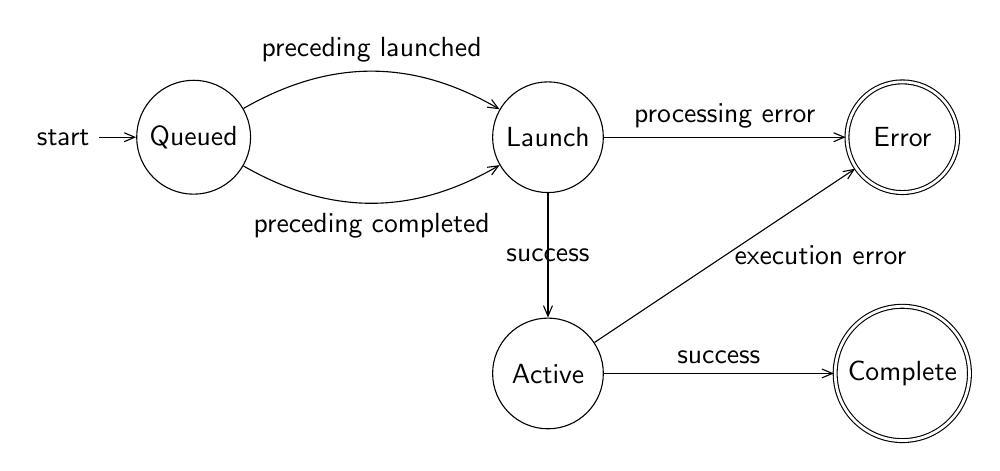
\begin{tikzpicture}
[auto,on grid,node distance=4.5cm,state/.style={circle,draw,minimum size=40pt}]
   \node[state,initial]                 (s0) {Queued};
   \node[state,right=4.5cm of s0]       (s1) {Launch};
   \node[state,below=3cm of s1]       (s2) {Active};
   \node[state,accepting,double distance=1pt,right=of s1]   (s3) {Error};
   \node[state,accepting,double distance=1pt,right=of s2]   (s4) {Complete};
   \path[->]
     (s0) edge[bend right]  node[below] {preceding completed} (s1)
          edge[bend left] node[above]{preceding launched} (s1)
     (s1) edge  node {processing error} (s3)
          edge  node[anchor=center] {success} (s2)
     (s2) edge  node{success} (s4)
          edge  node[right]{execution error} (s3)
     ;
\end{tikzpicture}
  \centering
  \caption{Packet State Diagram}
  \label{fig:packetstate}
\end{figure}

\begin{description}[leftmargin=0cm, labelindent=0cm]
\item[Queued] The queued state means that the format of the packet is not
  \hsaref{HSA_AQL_PACKET_FORMAT_ALWAYS_RESERVED} nor
  \hsaref{HSA_AQL_PACKET_FORMAT_INVALID}.  If the \reffld{barrier} bit is set, 
  the transition to launch state occurs after all the preceding kernels have 
  completed execution. If the \reffld{barrier} bit is not set, then the 
  transition to launch state occurs after the preceding kernels have completed 
  their launch phase.

\item[Launch] The launch state indicates processing of the packet, but not
  execution of a task. This phase finalizes by applying an acquire memory fence.
  If an error is detected during launch, the queue is set into an error state
  and the event callback associated with the queue (if present) is invoked. The
  following error might be communicated during the launch
  phase:\begin{inparaenum}[a\upshape)]\item
    \hsaref{HSA_STATUS_ERROR_INVALID_PACKET_FORMAT}, if the AQL packet is
    malformed\end{inparaenum}.

\item[Active] The active state means that the kernel encoded by the packet 
  has started execution. If an error is detected during this phase, a release 
  fence is applied to the packet and its completion signal (if present) is 
  assigned a negative value.

\item[Error] The error state means that an error was encountered during the 
  launch or active phases.

\item[Complete] The complete state means that a memory release fence has been
  applied and the completion signal (if present) decremented.
\end{description}

\subsubsection{Segment sizes}\label{segment-sizes}

If the kernel being dispatched uses private or group segments, the HSA runtime 
requires the application to specify the sizes of the segments in the Dispatch
packet. Manually calculating this information is not feasible and requires
visual inspection of the input program, which itself may have been generated by a
higher-level compiler. For this reason, the user must rely on the finalizer to get the
corresponding segment sizes. For more information on determining segment sizes, 
refer to Section~\ref{finalizerchapter}.

Another kind of HSA segment is the kernarg segment. It is also a part of the 
Dispatch packet; specified as a pointer. The kernarg segment data field 
specifies the arguments required to execute the kernel being dispatched. The 
application must specify this information. The layout of this segment is 
language/finalization specific and associated with the code object generated by 
finalization) prior to writing the AQL packet to the queue. This is unlike the 
group and private segments, whose lifespan spans only the active state of the 
Dispatch packet). % Please refer to the HSAIL
% service layer \mariotodo{missing} for an example on how to setup the kernarg
% segment for the HSAIL language, which is based on the 32/64 bit modes the kernel
% is compiled in.

\subsection{Agent Dispatch packet}\label{agent-packet}

Agent Dispatch packets dispatch jobs to HSA agents. The HSA API defines type 
\hsaref{hsa_aql_agent_dispatch_packet_t} to represent Agent Dispatch packets. 
The states and state transitions for Agent Dispatch packets is identical to that 
of Dispatch packets.

\subsection{Barrier packet}\label{barrier-packet}

The Barrier packet \hsaref{hsa_aql_barrier_packet_t} allows an application to 
specify up to five dependencies as \hsaref{hsa_signal_handle_t} objects and 
requires the HSA Packet Processor to resolve those dependencies before proceeding. 
The Barrier packet is a blocking packet in the sense that the processing of the 
Barrier packet completes the packet. This is unlike a Dispatch packet whose 
completion may occur at some future time after the packet has finished 
processing.

The HSA Packet Processor will not launch any further packets until the Barrier 
packet is complete. The execution phase for the Barrier packet completes when 
either of these two conditions have been met:
\begin{itemize}
\item Any of the dependent signals have been observed with a negative value 
  after the Barrier packet launched, in which case the HSA Packet 
  Processor assigns an error value to the \reffld{completion_signal} .
\item All of the dependent signals have been observed with the value 0 after 
  the Barrier packet launched (note that it is not required that all dependent 
  signals are observed to be 0 at the same time).
\end{itemize}

As stated above, if any of the dependent signals have been assigned a negative 
value, the Barrier packet will indicate failure in its completion signal. The 
HSA Packet Processor assigns an error value to the \reffld{completion_signal}. 
For more information, refer to Section~\ref{sec:signals}.

The state diagram of the Barrier packet is identical to that shown for Dispatch
packets. However, each state might cause a different set of actions:
\begin{itemize}
\item No memory fence is applied in the launch phase.
\item In the active phase, instead of executing a kernel, the packet waits for
  all the conditions to be met. The following errors might be communicated
  during the active phase: \begin{inparaenum}[a\upshape)]\item
    \hsaref{HSA_STATUS_ERROR_SIGNAL_DEPENDENCY}, if an error is detected in one
    of the dependent signals (a negative value is observed).\end{inparaenum}
\item No action is performed in the completion phase.
\end{itemize}

\subsection{API}
\input{api/altlatex/group-aql}

\section{Memory}\label{memory}\hypertarget{memory}{}

One of the key features of HSA is its ability to share global pointers between
the host application and code executing on the component. This ability means
that an application can directly pass a pointer to memory allocated on the host
to a kernel function dispatched to a component without an intermediate copy.

\hypertarget{memory-registration}{}\subsection{Registration}\label{memory-registration}

When a buffer will be accessed by a kernel running on a HSA device, programmers
are encouraged to register the corresponding address range beforehand by using
the appropriate HSA core API invocation. While kernels running on HSA devices
can access any valid system memory pointer allocated by means of standard
libraries (for example, malloc in the C language) without resorting to
registration, there might be a performance benefit from registering the buffer
with the HSA core component. When an HSA program no longer needs to access a
registered buffer in a device, the user should deregister that virtual address
range by using the appropriate HSA core API invocation.


\subsection{Global  Memory Allocation}\label{globalmemory}

While a HSA component is capable of accessing pageable system memory by
definition, for scenarios where wants memory allocated that has already been
registered (combine the allocation with memory registration), the HSA runtime
provides an interface, \hsaref{hsa_memory_allocate} to allocate memory that is
internally registered by the runtime:


\hypertarget{kernarg}{}\subsection{Kernarg Memory}\label{kernargmem}

The kernarg memory that AQL packet points to (see Section~\ref{sec:aql}) holds
information about any arguments required to execute AQL dispatch on a HSA
component. While any system memory may be used for kernarg memory,
implementation/platform specific optimizations are possible if HSA core runtime
provided API are utilized for allocating and copying to the allocated kernarg
memory.

\hypertarget{device-memory}{}\subsection{Component Local Memory}
\label{device-memory}

Component local memory is a memory type that is dedicated specifically for a
particular HSA component. This memory could provide higher bandwidth for
component access (than system memory) with the limitation that the host might
not be able to access it directly. HSA runtime provides a host interface to
allocate/deallocate and access component local memory. The user should not
register or deregister component local memory.

\subsection{API}
\input{api/altlatex/group-memory}

\subsection{Example - memory registration}

A buffer is registered by indicating its starting address and a size. The size
does not need to match that of the original allocation. For example:

\begin{lstlisting}
void* ptr = malloc(16);
status = hsa_memory_register(ptr, 8);
if(status == HSA_STATUS_ERROR_INVALID_ARGUMENT)
  handle_error(status);
\end{lstlisting}

is a valid program. On the other hand:

\begin{lstlisting}
void* ptr = malloc(16);
status = hsa_memory_register(ptr, 20);
if(status == HSA_STATUS_ERROR_INVALID_ARGUMENT)
  handle_error(status);
\end{lstlisting}

is not a valid program, because we are registering a range that spans several
allocations, or might not be entirely allocated.

Registrations can overlap previously registered intervals. A special case of
overlapped registrations is multiple registration. If the same interval is
registered several times with different sizes, the HSA core component will
select the maximum as the size of all the registrations. Therefore, the
following program:

\begin{lstlisting}
status = hsa_memory_register(ptr, 8);
if(status == HSA_STATUS_ERROR_INVALID_ARGUMENT)
  handle_error(status);
status = hsa_memory_register(ptr, 16);
if(status == HSA_STATUS_ERROR_INVALID_ARGUMENT)
  handle_error(status);
\end{lstlisting}

behaves identically to this program:

\begin{lstlisting}
hsa_memory_register(ptr, 16);
if(status == HSA_STATUS_ERROR_INVALID_ARGUMENT)
  handle_error(status);
hsa_memory_register(ptr, 16);
if(status == HSA_STATUS_ERROR_INVALID_ARGUMENT)
  handle_error(status);
\end{lstlisting}

While the described behavior might seem counter-intuitive, consider the
following scenario: A pointer is registered twice with different sizes s1 and
s2. When the pointer is deregistered, which interval should be deregistered: (p,
s1) or (p, s2)? If all the registrations of the same pointer are considered
identical by the core runtime, that problem is eliminated.

Deregistering a pointer that has not been previously registered results in an
\emph{info} status indicating the same.

The following code snippet revisits the introductory example. The code is almost
identical to the original, except that we register the buffers that will be
accessed from the device after allocating them, and we deregister all that
memory before releasing it. In some platforms, we expect this version to perform
better than the original one.

\subsection{Example - device memory}
Component memory is allocated by indicating the size and the HSA device it
corresponds to. For example, the following code allocates 1024 bytes of device
local memory:

\begin{lstlisting}
void* component_ptr = NULL;
hsa_memory_allocate_component_local(1024, component, &component_ptr);
\end{lstlisting}

To access component memory from the host, the user can call
\hsaref{hsa_memory_copy_component_local_to_system} in similar fashion as in
memcpy. This interface allows the user to perform component-to-host memory
copy. For example:

\begin{lstlisting}
 const size_t DATA_SIZE = 1024;
 void* src_ptr = malloc(DATA_SIZE);
 void* dest_ptr = NULL;
 hsa_memory_allocate_component_local(DATA_SIZE, device, &dest_ptr);
 hsa_memory_copy_component_local_to_system(dest_ptr, src_ptr, DATA_SIZE);
\end{lstlisting}

copies 1024 bytes from system to component local memory.


% \hypertarget{agent}{}\section{Agent Dispatch}\label{agent}
% The core runtime supports agent dispatches from an HSA agent. The
% runtime defines a default service queue for every user mode queue created by the
% user. This default service queue is available to the HSAIL programs and the user
% applications may submit agent dispatch packets to the service queue or any user
% mode queue. The service queue shares the same structure as the regular HSA
% queue. The default service queues are monitored by the
% runtime.

% \subsection{API}
% \input{api/altlatex/group-agent-dispatch}


\section{Extensions to the Core Runtime API}\label{extensions}

Extensions to the Core API can be optional (multi-vendor) or vendor
specific. The difference is in the naming scheme used for the symbols (defines,
structures, functions, etc.) associated with the function:

\begin{itemize}
\item Symbols for multi-vendor extensions defined in the global namespace must
  use the \emph{hsa_ext_} prefix in their identifiers.
\item Symbols for single vendor extensions defined in the global namespace must
  use the \emph{hsa_svext_VENDOR_} prefix in their identifiers. Company names
  must be registered with the HSA Foundation, must be unique, and may be
  abbreviated to improve the readability of the symbols.
\end{itemize}

Any constant definitions in the extension (\#define or enumeration values) use
the same naming convention, except using all capital letters.

The symbols for all vendor extensions (both single-vendor and multi-vendor) are
captured in the file {\bf hsa/vendor_extensions.h}. This file is maintained by
the HSA Foundation. This file includes the enumeration \hsaref{hsa_extension_t}
which defines a unique code for each vendor extension and multi-vendor
extension. Vendors can reserve enumeration encodings through the HSA
Foundation. Multi-vendor enumerations begin at the value of
\hsaref{HSA_EXT_START}, while single-vendor enumerations begin at
\hsaref{HSA_SVEXT_START}

\subsection{API}
\input{api/altlatex/group-extensions}

\subsection{Example}
An example that shows a hypothetical single-vendor extension ``Foo'' registered
by company ``ACME''. The example includes four defines and two API functions.
Note the use of the structure \reftyp{hsa_svext_acme_foo_t} and how this
interacts with the \hsaref{hsa_vendor_extension_query} API call.

\lstinputlisting{example/extension.c}

\section{Common Definitions}\label{sec:other}
\input{api/altlatex/group-RuntimeCommon}
%\input{api/altlatex/group-clock}


\chapter{HSA Extensions Programming Guide}

\section{HSAIL Finalization}
\label{finalizerchapter} \hypertarget{finalizerchapter}{}

The following subsections have to be updated according to the API definitions
introduced in version 0.180 of the specification.


% Compilation support in the HSA core runtime comprises of a finalization
% step. The primary functionality of this step is to translate the HSAIL to a
% component specific instruction set and produce a compilation unit. It resolves
% user defined symbols that are not already bound via callbacks provided by the
% user.

% HSA components may support HSAIL natively or may have a native ISA that the
% HSAIL needs to be translated into. However, compilation is a necessary step and
% is required despite a HSA components' native support of HSAIL. This is because
% of two primary reasons:

% \begin{enumerate}
% \item The HSA kernel code objects (accessible via the
%   \hsaref{hsa_compilationunit_code_t} structure, discussed in
%   Section~\ref{finalize:codeobject} ) are an output of the finalization process
%   and required as an input for the AQL Dispatch packet; to obtain values from
%   the finalizer for segment sizes etc.\ and also to act as a container for
%   component specific execution information.

% \item In order to support kernel dispatches from the HSA component, the kernel
%   code object must reside in a memory layout specification since dispatches
%   initiated from components are able to use memory operations to get the
%   information necessary for a dispatch.
% \end{enumerate}

% \subsubsection{BRIG and .directive Section}
% The core runtime accepts HSAIL programs coded in the BRIG binary format, as
% defined in the HSA PRM~\cite{prm}, for its finalization process. BRIG is a
% binary format defined by the HSA PRM and includes 5 different sections,
% \emph{.string}, \emph{.directive}, \emph{.code}, \emph{.operand}, and
% \emph{.debug}. More information on these sections is described in Section 19.1
% of the HSA PRM. The core runtime structure that represents a BRIG is named
% \hsaref{hsa_brig_t}. This structure is an in-memory representation of the
% BRIG. It is defined as follows:

% [DELETED CODE]

% Of the different sections in BRIG, the .directive section provides information
% to the finalizer on functions, kernels, and global declarations, etc. The
% symbols in the .directive section have defined placement rules (see PRM for more
% information). For example, immediately after a function or kernel directive,
% BRIG requires the directives that describe the arguments to be in a certain
% order. Return arguments are first, followed by input arguments, followed by the
% directives that apply only to the function or kernel.

% The \hsaref{hsa_brig_t} structure has the base address of the directive
% section. A directive for any symbol is represented using an offset into the
% directive section. HSA core runtime defines a type
% \hsaref{hsa_brig_directive_offset_t} to represent the .directive section
% offset. It is typedef to an unsigned 32 bit integer and is defined by all
% implementations as follows:

% [DELETED CODE]

% There are different types of directives specified in the PRM. Of these, the
% control directives are a means to allow implementations to pass information to
% the finalizer via HSAIL. HSA runtime defines a structure
% \hsaref{hsa_control_directives_t} to represent the values of control
% directives both at finalization time and to record information in the kernel
% code object. Control directives may also be specified within the HSAIL
% code. When conflicting values are specified for a particular directive specified
% in HSAIL and at finalization time, the runtime will do one of the following: (a)
% perform a union (OR operation) when possible (e.g. when the value represents a
% bit field).

% (b) when a union is not meaningful, the runtime will require that the value
% provided at finalization time via the \hsaref{hsa_control_directives_t}
% structure match the value for this directive in the HSAIL kernel.

% The \hsaref{hsa_control_directives_t} structure is defined as
% follows:

% [DELETED CODE]

% Where, the \hsaref{hsa_control_directive_present64_t} is defined as a 64bit
% unsigned integer.
% [DELETED CODE]

% The enumeration \hsaref{hsa_control_directive_present64_t} is a bit set
% indicating which control directives have been specified. It is accessible via a
% mask, \hsaref{hsa_control_directives_present_mask_t}, which is defined as
% follows:

% [DELETED CODE]

% User can choose to either break on exceptions or just detect them. The PRM
% defines the policy to be exception-type specific, i.e.\ different IEEE
% exceptions supported by HSA (see the definition of the enumeration
% \hsaref{hsa_exception_kind_mask_t} below) can be handled with different
% policies (BREAK vs.\ DETECT). The \reffld{enable_break_exceptions} field
% specifies the set of HSAIL exceptions that must have the BREAK policy
% enabled. It is possible that on some systems, enabling exceptions may result in
% lower code performance. If the kernel being finalized has any
% \texttt{enablebreakexceptions} control directives in HSAIL, then the runtime
% performs a union (OR operation) of values specified by this argument with the
% values in HSAIL control directives. If any of the functions the kernel calls
% have an enablebreakexceptions control directive, then they must be equal to or a
% subset of this union.

% [DELETED CODE]

% \subsubsection{Code Objects}\label{finalize:codeobject}

% There are different code objects defined by the runtime specification in support
% of HSAIL: \hsaref{hsa_kernel_code_t}, \hsaref{hsa_compilationunit_code_t}
% and \hsaref{hsa_function_code_t}. All of them are in memory and can be
% relocatable and/or position independent (which indicates that the object can be
% deep-copied to other memory locations for execution). The HSA runtime provides a
% query API to verify if a particular component supports position independent code
% objects (see Section~\ref{topology}).

% The \hsaref{hsa_compilationunit_code_t} is the header for the code object
% produced by the Finalizer and contains information that applies to all code
% entities in the compilation unit.

% Since core runtime does not define a file format container, the core runtime
% provides API to work with HSAIL programs encoded in the BRIG binary format and
% supports generation of code objects that include kernels to be executed in the
% HSA component and binding of unresolved symbols associated with the code object
% generated.

% Finalizer allocates a single contiguous area of memory to hold the generated
% code for all the code objects.

% The structure of this contiguous area is as follows: Starting at offset 0, the
% ``header'' of this contiguous area is defined by the
% \hsaref{hsa_compilationunit_code_t} structure. The
% \hsaref{hsa_compilationunit_code_t} structure in turn contains an offset to
% an array of \hsaref{hsa_code_entry_t}, one entry per code entity that the
% finalizer has produced code for. Each \hsaref{hsa_code_entry_t} variable
% contains an offset to a \hsaref{hsa_*code_t} object that describes that code
% entity (function/kernel/etc).

% [DELETED CODE]

% Every \hsaref{hsa_*_code_t} code objects start with a common header that also
% contains what kind of code object it is. The common header,
% \hsaref{hsa_code_t}, is defined as follows:
% [DELETED CODE]

% A bit set of flags providing information about the code in a compilation
% unit. Unused flags must be 0. The \hsaref{hsa_code_properties32_t} must be
% used as a type for this flag. The values/mask currently supported is defined as
% follows:
% [DELETED CODE]

% The \hsaref{hsa_compilationunit_code_t} structure is defined as
% follows:
% [DELETED CODE]

% Both the \hsaref{hsa_compilationunit_t} and \hsaref{hsa_*_code_t} objects
% can have implementation define data towards the end of the structure. All
% elements in the contiguous location being accessed by offsets enables such
% definition. This also allows the exact position of the various objects in the
% contiguous memory area to be implementation defined as long as memory alignment
% requirements are met.

% Many of the \hsaref{hsa_*_code_t} objects include a size field which is
% required to be set to the size of the structure. This allows forward
% compatibility and allows for structure definitions to change or include
% implementation specific information.

% The \hsaref{hsa_kernel_code_t} is required for all component dispatches and
% is referred to by the dispatch AQL packets placed in the HSA queue. This allows
% an implementation to rely on all such objects being the same size for more
% efficient navigation to the implementation specific data without need to first
% read the object's size field.

% The \hsaref{hsa_kernel_code_t} is the output of
% \hsaref{hsa_finalize_brig} API and is defined as follows.
% [DELETED CODE]

% \subsubsection{Finalize BRIG API}
% The \hsaref{hsa_finalize_brig} API accepts \hsaref{hsa_brig_t} as an input
% and produces relocatable code object in which global and group symbols are bound
% to actual, component recognizable, addresses. A symbol in the finalization step
% can be a variable, a function, image or a sampler. When finalization occurs, a
% \hsaref{hsa_kernel_code_t}, representing the kernel that needs to be executed
% on the component is generated. However, all the symbols referenced in the
% kernel being finalized may not be resolved with the information provided at its
% finalization. User is allowed to define callbacks that can resolve the symbols
% declared in the global segment, with the following signature:
% [DELETED CODE]

% The finalization step, when successfully executed, can have two distinct
% outputs. The first is the compilation unit code object,
% \hsaref{hsa_compilationunit_code_t} which is discussed in
% Section~\ref{finalize:codeobject}. The second output is of type
% \hsaref{hsa_compilationunit_debug_t} which is only generated when the code is
% compiled with a debug option. This debug information is currently implementation
% defined.

% Since the contiguous memory that {\itshape compilationunit_code} represents and
% the memory for {\itshape compilationunit_debug} need to be allocated, the user
% is expected to provide callbacks for memory allocation.

% The callback is required to have the following signature:
% [DELETED CODE]

% Where caller is the opaque pointer passed to the \hsaref{hsa_finalize_brig}
% that is calling back this function. {\itshape byte_size} is the size in bytes
% of the memory to be allocated. {\itshape byte_alignment} is the required byte
% alignment of the memory allocated. Must be a power of 2. {\itshape address} is
% pointer to location that will be updated with address of allocated memory if
% successful, or NULL if not successful. {\itshape return value} is the HSA
% status of the allocation.
% [DELETED CODE]

% HSAIL does not define a set of options that a finalizer needs to specify. To
% ensure portability, \hsaref{hsa_finalize_brig} must not return an error status
% if a given compilation option is not recognized.

% The callback for the allocation of \hsaarg{compilationunit_debug} is optional
% and is required when the user passes in a flag at finalization to generate debug
% information. This callback, when defined, must have the same signature as
% \hsaref{hsa_alloc_t} above.

% \subsubsection{Freeing The Compilation Unit Code/Debug Object}
% The core runtime also provides a corresponding destruction API that destroys the
% compilation unit code and debug objects. This will reclaim all memory used by
% the \hsaref{hsa_compilationunit_code_t} (including the ISA it contains) and
% associated \hsaref{hsa_compilationunit_debug_t}. It will also unregister the
% ISA memory if appropriate.

% [DELETED CODE]

% Note that destroying does not impact any memory segments that may have been
% allocated/reserved for use in a kernel from this object. It merely releases
% resources used to build the object.

% \subsubsection{Serializing and Deserializing a Compilation Unit}

% Because of the opaque nature of what the compilation unit actually represents,
% and in order for the users of the core runtime to build file containers,
% serialization and deserialization API are defined by the core runtime. The
% definition is as follows:

% [DELETED CODE]

\subsection{API}
\input{api/altlatex/group-FinalizerCoreApi}

%\subsection{Group Memory Usage}\label{groupmem}

% Group memory can be allocated either
% statically when the finalizer is called or dynamically by the user at launch
% time.

% Static allocation is supported as follows:
% \begin{itemize}
% \item The \hsaref{hsa_finalize_brig} routine writes the amount of group memory
%   needed by the finalized ISA to the
%   \hsaref{hsa_code_descriptor_t}.\reffld{workgroup_group_segment_size_byte}
%   field. The group memory usage includes group memory which is statically
%   allocated in the HSAIL kernel, as well as private group memory used by the
%   finalizer. Different HSA implementations might allocate different amounts of
%   group memory.

% \item The user copies the requested group segment usage to the Dispatch packet
%   field \reffld{group_segment_size_bytes}.

% \item The packet processor reads the group memory usage field and reserves the
%   required resources at dispatch time.

% \item Statically allocated group memory starts at a segment offset of 0.

% \end{itemize}

% Dynamically allocated group memory allows the user to specify the group memory
% size when the kernel is launched. This is useful to support dynamic group memory
% allocation features supported by languages such as OpenCL. Essentially, the user
% manually calculates the offset for each kernel argument (including the static
% allocation in the calculation) and passes these as arguments to the HSAIL
% kernel. Specifically:

% \begin{itemize}

% \item As above, the \hsaref{hsa_finalize_brig} routine returns the requested
%   static group allocation.

% \item HSAIL will use standard 32-bit arguments (that is, \ttbf{kernarg_u32})
%   to specify group segment offsets. The user is responsible for computing the
%   offset for each group memory argument location. The first argument must start
%   just above the static allocation, so it always has the offset of
%   \reffld{workgroup_group_segment_size_byte} (see
%   \hsaref{hsa_code_descriptor_t}).

% \item After setting the offset for each group memory argument, the user must set
%   the AQL Dispatch packet's \hsaref{hsa_aql_dispatch_packet_t}.\reffld{
%     group_segment_size_bytes} field to the total amount of group memory used
%   (static and dynamic allocations).

% \end{itemize}

% See below for an example of setting up dynamic group memory arguments for a
% kernel.  \lstinputlisting{example/group-sample.c}

% Here is the corresponding kernel and usage model:
% \lstinputlisting{example/group-sample-hsail.c}

\section{HSAIL Linking}\label{linking}
\subsubsection{API}
\input{api/altlatex/group-HsailLinkerServiceLayer}


\section{Images and Samplers}
\label{images} \hypertarget{images}{}

An HSA runtime uses an image handle \hsaref{hsa_ext_image_handle_t} to access 
images. The image handle references the image data in memory and records 
information about resource layout and other properties. HSA decouples the 
storage of the image data and the description of how the device interprets that 
data. This allows the application developer to control the location of the 
image data storage and manage memory more efficiently.

The HSA image format is specified using a format descriptor
(\hsaref{hsa_ext_image_format_t}) that contains information about the image
channel type and the channel order. The image channel type describes how the
data is to be interpreted along with the bit size, and image channel order
describes the number and the order. Not all image channel types and channel
order combinations are valid on a HSA agent. All HSA agents have to support a
required minimum set of image formats. For more information, refer to the HSA 
Programmer's Reference Manual\cite{prm}. An application can use 
\hsaref{hsa_ext_image_get_format_capability} to query a runtime 
to obtain image format capabilities.

An implementation-independent image format descriptor
(\hsaref{hsa_ext_image_descriptor_t}) is composed of geometry along with the
image format. The image descriptor is used to inquire the runtime for the HSA
component-specific image data size and alignment details by calling
\hsaref{hsa_ext_image_get_info} for the purpose of determining the
implementation's storage requirements.

The memory requirements (\hsaref{hsa_ext_image_info_t}) include the size of the
memory needed as well as any alignment constraints. An application can either
allocate new memory for the image data, or sub-allocate a memory block from an
existing memory if the memory size allows. Before the image data is used, an HSA
agent-specific image handle must be created using it and if necessary, cleared
and prepared according to the intended use.

A HSA agent-specific image handle (\hsaref{hsa_ext_image_handle_t}) is used by
the HSAIL language for reading or writing using HSAIL \refhsl{rd image},
\refhsl{ldimage} and \refhsl{stimage}
operations. \hsaref{hsa_ext_image_create_handle} creates an image handle from a
implementation-independent image format descriptor and independently allocated
image data that conforms to the requirements provided by
\hsaref{hsa_ext_image_get_info}.

It must be noted that while the image data technically accessible from its
pointer in the raw form, the data layout and organization is agent-specific and
should be treated as opaque. The internal implementation of an optimal image
data organization could vary depending on the attributes of the image format
descriptor. As a result, there are no guarantees on the data layout when
accessed from another HSA agent. The only reliable way to import or export image
data from optimally organized images is to copy their data to and from a
linearly organized data layout in memory, as specified by the image's format
attributes.

The HSA Runtime provides interfaces to allow operations on images. Image data
transfer to and from memory with a linear layout can be performed using
\hsaref{hsa_ext_image_export} and \hsaref{hsa_ext_image_import} respectively. A
portion of an image could be copied to another image using
\hsaref{hsa_ext_image_copy}. An image can be cleared using
\hsaref{hsa_ext_image_clear}. It is the application's responsibility to ensure
proper synchronization and preparation of images on accesses from other image
operations. See HSA System Architecture spec 2.13 for the HSA Image memory
model.

A HSA agent-specific sampler handle (\hsaref{hsa_ext_sampler_handle_t}) is used
by the HSAIL language to describe how images are processed by the
\refhsl{rdimage} HSAIL operation. \hsaref{hsa_ext_sampler_create_handle} creates
a sampler handle from an agent independent sampler descriptor
(\hsaref{hsa_ext_sampler_descriptor_t}).

\subsection{API}
\input{api/altlatex/group-images}

\section{Component Initiated Dispatches} \label{architected}
\hypertarget{architectedchptr}{}
%% \hyperlink{coreapi}{Core A\-P\-I
Documentation}\hypertarget{coreapi_dtde}{}\section{Component-\/\-Initiated
Dispatch}\label{coreapi_dtde}

Due to architected support for a queue and design of A\-Q\-L,
H\-S\-A supports component-\/initiated dispatch, which is the ability
for a kernel to dispatch a new kernel by writing an A\-Q\-L packet
directly to a user queue. In simple use cases, the A\-Q\-L packet
can be created on the host and passed as a parameter to the kernel.
This eliminates the need to do dynamic memory allocation on the
component, but has the limitation that the problem fanout must be known
at the time the first kernel is launched (so that the A\-Q\-L
packets can be preallocated). H\-S\-A also supports more advanced
use cases where the A\-Q\-L packet is dynamically allocated
(including the memory space for kernel arguments and
spill/arg/private space) on the component. This usage model obviously
requires dynamic component-\/side memory allocation, for both host and
component memory.

Some requirements to do component-\/initiated dispatch\-:

\begin{itemize}

\item Ability to dynamically choose a kernel to dispatch\-: Let us
assume for example that there are three kernels (A, B and C). If the
host launches A, then the user has the choice of launching B or C,
or even A in case of recursion. So, the user should be able to get
the I\-S\-A and segment size (Hsa\-Aql\-Kernel) from the
corresponding B\-R\-I\-G dynamically. \mbox{[}caveat\-: The code
sample here does not show how we can do this. It assumes that the
Hsa\-Aql\-Kernel is being passed as an argument to the parent kernel
(A in this case)\mbox{]}

\item Ability to dynamically allocate memory from the shader\-: We
need to allocate memory for A\-Q\-L\-Packet, different kernel
segments in the A\-Q\-L\-Packet, kernel arguments, and so forth.

\item Ability for a finalizer to identify a default H\-S\-A queue to
write A\-Q\-L\-Packet\-: The H\-S\-A queue information resides in
the runtime layer of the stack. This needs to be exchanged with the
compiler so it can be stored in the global space. This way, when the
compiler sees the queue, it knows where to pick the H\-S\-A queue
information to write the A\-Q\-L\-Packet.

\item Ability to notify the completion of all the
component-\/initiated dispatches on the host\-:

\begin{itemize}
\item The beginning of execution of the child kernel may or may not
wait for the parent kernel's completion. This is determined by the
user and could be algorithm dependent.
\item If the parent (initiated from host) kernel finishes
successfully, it means all kernels it initiated also finished
successfully.
\item To implement this, we need to track the list of kernels
launched from the parent. Change the status of parent to complete,
only if parent and all its child kernels have completed
successfully.
\end{itemize}
\end{itemize}

Implementations that support component initiated dispatches will
need to support these requirements. If the implementation supports
the stated requirements, the following actions will allow a
component to initiate a dispatch\-:
\begin{itemize}
\item The queue and \texttt{hsa\_code\_object\_t} (describing the
kernel to launch) can be passed as arguments to the parent (the one
launched from the host) kernel. If the dispatch is to the same
queue, it is accessible via an HSAIL instruction.
\item If not, get the Hsa\-Aql\-Kernel from the B\-R\-I\-G for the
kernel that is chosen to be dynamically dispatchd.
\item When new work is to be created, the H\-S\-A\-I\-L code would\-:
\begin{itemize}
\item Use the kernel dynamic memory allocator to allocate a new
A\-Q\-L\-Packet.
\item Use inline H\-S\-A\-I\-L to replicate the functionality of the
Hsa\-Init\-A\-Q\-L\-Packet function. We could perhaps provide an
H\-S\-A\-I\-L library to implement this functionality. Recall this
function\-:
\begin{itemize}
\item Copies some fields from the Hsa\-Aql\-Kernel structure (for
example, the kernel I\-S\-A) to the A\-Q\-L\-Packet
\item Uses a host allocator to allocate memory for the kernel
arguments
\item Uses a component allocator to allocate memory for spill,
private, and arg segments
\end{itemize}
\end{itemize}
\item The H\-S\-A\-I\-L knows the signature of the called function
and can fill in the A\-Q\-L packet with regular H\-S\-A\-I\-L global
store instructions.
\item The H\-S\-A queue is architected, so the H\-S\-A\-I\-L can use
memory store instructions to dispatch the kernel for dispatch.
Depending how the user queues are configured, atomic accesses might
be necessary to handle contention with other writers. Note that, if
the queue information is not passed in as an argument, the default
queue can be chosen by the finalizer as it was exchanged earlier
from the runtime layer.
\item We also need to handle deallocation of the kernel arguments
and spill/private/arg space after the kernel completes.
\item On the host, check if the parent has finished. If the parent
has finished successfully, then it means that all the child kernels
have finished successfully too. If the parent or any of the child
kernels failed, an error code will be returned. 
\end{itemize}


Due to architected support for a queue and design of AQL, HSA supports
component-initiated dispatch, which is the ability for a kernel to dispatch a
new kernel by writing an AQL packet directly to a user queue. In simple use
cases, the AQL packet can be created on the host and passed as a parameter to
the kernel. This eliminates the need to do dynamic memory allocation on the
component, but has the limitation that the problem fanout must be known at the
time the first kernel is launched (so that the AQL packets can be
preallocated). HSA also supports more advanced use cases where the AQL packet is
dynamically allocated (including the memory space for kernel arguments and
spill/arg/private space) on the component. This usage model obviously requires
dynamic component-side memory allocation, for both host and component memory.

Some requirements to do component-initiated dispatch:
\begin{itemize}
\item Ability to dynamically choose a kernel to dispatch: Let us assume for
  example that there are three kernels (A, B and C). If the host launches A,
  then the user has the choice of launching B or C, or even A in case of
  recursion. So, the user should be able to get the ISA and segment size
  (Hsa\-Aql\-Kernel) from the corresponding BRIG dynamically. \mbox{[}caveat:
  The code sample here does not show how we can do this. It assumes that the
  Hsa\-Aql\-Kernel is being passed as an argument to the parent kernel (A in
  this case)\mbox{]}

\item Ability to dynamically allocate memory from the shader: We need to
  allocate memory for AQL\-Packet, different kernel segments in the AQL\-Packet,
  kernel arguments, and so forth.

\item Ability for a finalizer to identify a default HSA queue to write
  AQL\-Packet: The HSA queue information resides in the runtime layer of the
  stack. This needs to be exchanged with the compiler so it can be stored in the
  global space. This way, when the compiler sees the queue, it knows where to
  pick the HSA queue information to write the AQL-Packet.

\item Ability to notify the completion of all the component-initiated
  dispatches on the host:

\begin{itemize}
\item The beginning of execution of the child kernel may or may not wait for the
  parent kernel's completion. This is determined by the user and could be
  algorithm dependent.
\item If the parent (initiated from host) kernel finishes successfully, it means
  all kernels it initiated also finished successfully.
\item To implement this, we need to track the list of kernels launched from the
  parent. Change the status of parent to complete, only if parent and all its
  child kernels have completed successfully.
\end{itemize}
\end{itemize}

Implementations that support component initiated dispatches will need to support
these requirements. If the implementation supports the stated requirements, the
following actions will allow a component to initiate a dispatch:
\begin{itemize}
\item The queue and \hsaref{hsa_ext_code_descriptor_t} (describing the kernel to
  launch) can be passed as arguments to the parent (the one launched from the
  host) kernel. If the dispatch is to the same queue, it is accessible via an
  HSAIL instruction.
\item If not, get the Hsa\-Aql\-Kernel from the BRIG for the kernel that is
  chosen to be dynamically dispatched.
\item When new work is to be created, the HSAIL code would:
\begin{itemize}
\item Use the kernel dynamic memory allocator to allocate a new AQL\-Packet.
\item Use inline HSAIL to replicate the functionality of the
  Hsa\-Init\-AQL\-Packet function. We could perhaps provide an HSAIL library to
  implement this functionality. Recall this function:
\begin{itemize}
\item Copies some fields from the Hsa\-Aql\-Kernel structure (for example, the
  kernel ISA) to the AQL\-Packet
\item Uses a host allocator to allocate memory for the kernel arguments
\item Uses a component allocator to allocate memory for spill, private, and arg
  segments
\end{itemize}
\end{itemize}
\item The HSAIL knows the signature of the called function and can fill in the
  AQL packet with regular HSAIL global store instructions.
\item The HSA queue is architected, so the HSAIL can use memory store
  instructions to dispatch the kernel for dispatch. Depending how the user
  queues are configured, atomic accesses might be necessary to handle contention
  with other writers. Note that, if the queue information is not passed in as an
  argument, the default queue can be chosen by the finalizer as it was exchanged
  earlier from the runtime layer.
\item We also need to handle deallocation of the kernel arguments and
  spill/private/arg space after the kernel completes.
\item On the host, check if the parent has finished. If the parent has finished
  successfully, then it means that all the child kernels have finished
  successfully too. If the parent or any of the child kernels failed, an error
  code will be returned.
\end{itemize}

% API index
\printindex[api]
\printindex[ext]

% inline bibliography for simplicity.
\bibliographystyle{plain}
\begin{thebibliography}{30}

\bibitem{prm}
HSA Foundation.
\newblock{The HSA Programmer's Reference Manual.}
\newblock{Technical report, HSA Foundation, 2013.}

\bibitem{sar}
HSA Foundation.
\newblock {The HSA Platform System Architecture Specification.}
\newblock{Technical report, HSA Foundation, 2014.}

\end{thebibliography}
% add bibliography to Table of Contents
\addcontentsline{toc}{chapter}{Bibliography}

\end{document}
